%!TEX encoding = UTF-8 Unicode
\documentclass[french, a4paper, 12pt]{article}



%% Langue et compilation

\usepackage[utf8]{inputenc}
\usepackage[T1]{fontenc}
\usepackage[french]{babel}

%% LISTE DES PACKAGES

\usepackage{mathtools}     % package de base pour les maths
\usepackage{amsmath}       % mathematical type-setting
\usepackage{amssymb}       % symbols speciaux pour les maths
\usepackage{textcomp}      % symboles speciaux pour el text
\usepackage{gensymb}       % commandes generiques \degree etc...
\usepackage{tikz}          % package graphique
\usepackage{wrapfig}       % pour entourer a cote d'une figure
\usepackage{color}         % package des couleurs
\usepackage{xcolor}        % autre package pour les couleurs
\usepackage{pgfplots}      % pacakge pour creer des graph
\usepackage{epsfig}        % permet d'inclure des graph en .eps
\usepackage{graphicx}      % arguments dans includegraphics
\usepackage{pdfpages}      % permet d'insérer des pages pdf dans le document
\usepackage{subfig}        % permet de creer des sous-figure
\usepackage{pst-all}       % utile pour certaines figures en pstricks
\usepackage{lipsum}        % package qui permet de faire des essais
\usepackage{array}         % permet de faire des tableaux
\usepackage{multicol}      % plusieurs colonnes sur une page
\usepackage{enumitem}      % pro­vides user con­trol: enumerate, itemize and description
\usepackage{hyperref}      % permet de creer des hyperliens dans le document
\usepackage{lscape}        % permet de mettre une page en mode paysage
\usepackage{lmodern}       % permet d'avoir certains "fonts" de bonen qualite
\usepackage{fancyhdr}      % Permet de mettre des informations en hau et en bas de page      
\usepackage[framemethod=tikz]{mdframed} % breakable frames and coloured boxes
\usepackage[top=1.5cm, bottom=1.5cm, left=2.5cm, right=2.5cm]{geometry} % donne les marges
\usepackage[font=normalsize, labelfont=bf,labelsep=endash, figurename=Fig.]{caption} % permet de changer les legendes des figures
\usepackage{lewis}
\usepackage{bohr}
\usepackage{chemfig}
\usepackage{chemist}

%% LIBRAIRIES

\usetikzlibrary{plotmarks} % librairie pour les graphes
\usetikzlibrary{patterns}  % necessaire pour certaines choses predefinies sur tikz
\usetikzlibrary{shadows}   % ombres des encadres
\usetikzlibrary{backgrounds} % arriere plan des encadres


%% MISE EN PAGE

\pagestyle{fancy}     % Défini le style de la page

\renewcommand{\headrulewidth}{1pt}      % largeur du trait en haut de la page
\fancyhead[L]{Seconde générale}         % info coin haut gauche
\fancyhead[R]{Lycée Jean Guéhenno}  % info coin haut droit

% bas de la page
\renewcommand{\footrulewidth}{1pt}      % largeur du trait en bas de la page
\fancyfoot[L]{G. \bsc{LE DOUDIC}}  % info coin bas gauche
\fancyfoot[R]{TP 4 : Famille chimique}                         % info coin bas droit


\setlength{\columnseprule}{1pt} 
\setlength{\columnsep}{30pt}



%% NOUVELLES COMMANDES 

\DeclareMathOperator{\e}{e} % permet d'ecrire l'exponentielle usuellement


\newcommand{\gap}{\vspace{0.15cm}}   % defini une commande pour sauter des lignes
\renewcommand{\vec}{\overrightarrow} % permet d'avoir une fleche qui recouvre tout le vecteur
\newcommand{\bi}{\begin{itemize}}    % begin itemize
\newcommand{\ei}{\end{itemize}}      % end itemize
\newcommand{\bc}{\begin{center}}     % begin center
\newcommand{\ec}{\end{center}}       % end center
\newcommand\opacity{1}               % opacity 
\pgfsetfillopacity{\opacity}

\newcommand*\Laplace{\mathop{}\!\mathbin\bigtriangleup} % symbole de Laplace

\frenchbsetup{StandardItemLabels=true} % je ne sais plus

\newcommand{\smallO}[1]{\ensuremath{\mathop{}\mathopen{}o\mathopen{}\left(#1\right)}} % petit o

\newcommand{\cit}{\color{blue}\cite} % permet d'avoir les citations de couleur bleues
\newcommand{\bib}{\color{black}\bibitem} % paragraphe biblio en noir et blanc
\newcommand{\bthebiblio}{\color{black} \begin{thebibliography}} % idem necessaire sinon bug a cause de la couleur
\newcommand{\ethebiblio}{\color{black} \end{thebibliography}}   % idem
%%% TIKZ


%% COULEURS 


\definecolor{definitionf}{RGB}{220,252,220}
\definecolor{definitionl}{RGB}{39,123,69}
\definecolor{definitiono}{RGB}{72,148,101}

\definecolor{propositionf}{RGB}{255,216,218}
\definecolor{propositionl}{RGB}{38,38,38}
\definecolor{propositiono}{RGB}{109,109,109}

\definecolor{theof}{RGB}{255,216,218}
\definecolor{theol}{RGB}{160,0,4}
\definecolor{theoo}{RGB}{221,65,100}

\definecolor{avertl}{RGB}{163,92,0}
\definecolor{averto}{RGB}{255,144,0}

\definecolor{histf}{RGB}{241,238,193}

\definecolor{metf}{RGB}{220,230,240}
\definecolor{metl}{RGB}{56,110,165}
\definecolor{meto}{RGB}{109,109,109}


\definecolor{remf}{RGB}{230,240,250}
\definecolor{remo}{RGB}{150,150,150}

\definecolor{exef}{RGB}{240,240,240}

\definecolor{protf}{RGB}{247,228,255}
\definecolor{protl}{RGB}{105,0,203}
\definecolor{proto}{RGB}{174,88,255}

\definecolor{grid}{RGB}{180,180,180}

\definecolor{titref}{RGB}{230,230,230}

\definecolor{vert}{RGB}{23,200,23}

\definecolor{violet}{RGB}{180,0,200}

\definecolor{copper}{RGB}{217, 144, 88}

%% Couleur des ref

\hypersetup{
	colorlinks=true,
	linkcolor=black,
	citecolor=blue,
	urlcolor=black
		   }

%% CADRES


% %%%%%%%%%% DEFINITION
% \newmdenv[tikzsetting={fill=definitionf}, linewidth=2pt, linecolor=definitionl, outerlinewidth=0pt, innertopmargin=5pt, innerbottommargin=5pt, innerleftmargin=5pt, innerrightmargin=5pt, leftmargin=0pt]{definition}

% \newmdenv[ tikzsetting={drop shadow={ shadow xshift=1ex, shadow yshift=-0.5em, fill=definitiono, opacity=1, every shadow } }, outerlinewidth=2pt, outerlinecolor=white, linecolor=white, innertopmargin=0pt, innerbottommargin=0pt, innerleftmargin=0pt, innerrightmargin=0pt]{ombredef}


% %%%%%%%%%% THEOREME

% \newmdenv[tikzsetting={fill=theof}, linewidth=2pt, linecolor=theol, outerlinewidth=0pt, innertopmargin=5pt, innerbottommargin=5pt, innerleftmargin=5pt, innerrightmargin=5pt, leftmargin=0pt]{theo}

% \newmdenv[ tikzsetting={drop shadow={ shadow xshift=1ex, shadow yshift=-0.5em, fill=theoo, opacity=1, every shadow } }, outerlinewidth=2pt, outerlinecolor=white, linecolor=white, innertopmargin=0pt, innerbottommargin=0pt, innerleftmargin=0pt, innerrightmargin=0pt]{ombretheo}


% %%%%%%%%%% METHODE

% \newmdenv[tikzsetting={fill=metf}, linewidth=2pt, linecolor=metl, outerlinewidth=0pt, innertopmargin=5pt, innerbottommargin=5pt, innerleftmargin=5pt, innerrightmargin=5pt, leftmargin=0pt]{met}

% \newmdenv[ tikzsetting={drop shadow={ shadow xshift=1ex, shadow yshift=-0.5em, fill=meto, opacity=1, every shadow } }, outerlinewidth=2pt, outerlinecolor=white, linecolor=white, innertopmargin=0pt, innerbottommargin=0pt, innerleftmargin=0pt, innerrightmargin=0pt]{ombremet}



%%%%%%%%%%% RQ

\newmdenv[tikzsetting={fill=remf}, linewidth=2pt, linecolor=remf, outerlinewidth=0pt, innertopmargin=5pt, innerbottommargin=5pt, innerleftmargin=5pt, innerrightmargin=5pt, leftmargin=0pt]{remarque}

\newmdenv[ tikzsetting={drop shadow={ shadow xshift=1ex, shadow yshift=-0.5em, fill=remo, opacity=1, every shadow } }, outerlinewidth=2pt, outerlinecolor=white, linecolor=white, innertopmargin=0pt, innerbottommargin=0pt, innerleftmargin=0pt, innerrightmargin=0pt]{ombreremarque}

%%%%%%%%%%% Cadre pour le titre

\tikzset{every shadow/.style={opacity=1}}

\global\mdfdefinestyle{doc}{backgroundcolor=white, shadow=true, shadowcolor=propositiono, linewidth=1pt, linecolor=black, shadowsize=5pt}
\global\mdfdefinestyle{titr}{backgroundcolor=metf, shadow=true, shadowcolor=propositiono, linewidth=1pt, linecolor=black, shadowsize=5pt}
\global\mdfdefinestyle{theo}{backgroundcolor=theof, shadow=true, shadowcolor=theoo, linewidth=1pt, linecolor=theol, shadowsize=5pt}
\global\mdfdefinestyle{prop}{backgroundcolor=theof, shadow=true, shadowcolor=propositiono, linewidth=1pt, linecolor=theol, shadowsize=5pt}
\global\mdfdefinestyle{def}{backgroundcolor=definitionf, shadow=true, shadowcolor=definitiono, linewidth=1pt, linecolor=definitionl, shadowsize=5pt}
\global\mdfdefinestyle{histo}{backgroundcolor=histf, shadow=true, shadowcolor=propositiono, linewidth=1pt, linecolor=black, shadowsize=5pt}
\global\mdfdefinestyle{avert}{backgroundcolor=white, shadow=true, shadowcolor=averto, linewidth=1pt, linecolor=avertl, shadowsize=5pt}
\global\mdfdefinestyle{met}{backgroundcolor=metf, shadow=true, shadowcolor=meto, linewidth=1pt, linecolor=metl, shadowsize=5pt}
\global\mdfdefinestyle{rem}{backgroundcolor=metf, shadow=true, shadowcolor=meto, linewidth=1pt, linecolor=metf, shadowsize=5pt}
\global\mdfdefinestyle{exo}{backgroundcolor=exef, shadow=true, shadowcolor=propositiono, linewidth=1pt, linecolor=exef, shadowsize=5pt}
\global\mdfdefinestyle{not}{backgroundcolor=definitionf, shadow=true, shadowcolor=propositiono, linewidth=1pt, linecolor=black, shadowsize=5pt}
\global\mdfdefinestyle{proto}{backgroundcolor=protf, shadow=true, shadowcolor=proto, linewidth=1pt, linecolor=protl, shadowsize=5pt}

%%%%%%
\definecolor{cobalt}{rgb}{0.0, 0.28, 0.67}
\definecolor{applegreen}{rgb}{0.55, 0.71, 0.0}

\usepackage{tcolorbox}
  \tcbuselibrary{most}
  \tcbset{colback=cobalt!5!white,colframe=cobalt!75!black}



\newtcolorbox{definition}[1]{
	colback=applegreen!5!white,
  	colframe=applegreen!65!black,
	fonttitle=\bfseries,
  	title={#1}}
\newtcolorbox{Programme}[1]{
	colback=cobalt!5!white,
  	colframe=cobalt!65!black,
	fonttitle=\bfseries,
  	title={#1}}  

\newtcolorbox{Exercice}[1]{
  colback=cobalt!5!white,
  colframe=cobalt!65!black,
  fonttitle=\bfseries,
  title={#1}}  

  \newtcolorbox{Protocol}[1]{
  colback=cyan!5!white,
  colframe=cyan!65!black,
  fonttitle=\bfseries,
  title={#1}}  

\newtcolorbox{Resultat}[1]{
	colback=theof,%!5!white,
	colframe=theoo!85!black,
  fonttitle=\bfseries,
	title={#1}} 	


\def\width{12}
\def\hauteur{5}

\setlength{\parskip}{0pt}%
\setlength{\parindent}{18pt}


%% MODIFICATION DE CHAPTER  
\makeatletter
\def\@makechapterhead#1{%
  %%%%\vspace*{50\p@}% %%% removed!
  {\parindent \z@ \raggedright \normalfont
    \ifnum \c@secnumdepth >\m@ne
        \huge\bfseries \@chapapp\space \thechapter
        \par\nobreak
        \vskip 20\p@
    \fi
    \interlinepenalty\@M
    \Huge \bfseries #1\par\nobreak
    \vskip 40\p@
  }}
\def\@makeschapterhead#1{%
  %%%%%\vspace*{50\p@}% %%% removed!
  {\parindent \z@ \raggedright
    \normalfont
    \interlinepenalty\@M
    \Huge \bfseries  #1\par\nobreak
    \vskip 40\p@
  }}
  
  \newcommand{\isotope}[3]{%
     \settowidth\@tempdimb{\ensuremath{\scriptstyle#1}}%
     \settowidth\@tempdimc{\ensuremath{\scriptstyle#2}}%
     \ifnum\@tempdimb>\@tempdimc%
         \setlength{\@tempdima}{\@tempdimb}%
     \else%
         \setlength{\@tempdima}{\@tempdimc}%
     \fi%
    \begingroup%
    \ensuremath{^{\makebox[\@tempdima][r]{\ensuremath{\scriptstyle#1}}}_{\makebox[\@tempdima][r]{\ensuremath{\scriptstyle#2}}}\text{#3}}%
    \endgroup%
  }%

\makeatother

\usepackage{eurosym}
\usepackage{colortbl}
%%
%% DEBUT DU DOCUMENT
%%
\begin{document}


%%%%%%

\titre{Chapitre 7: Lentilles et modèle optique de l'\oe il}

\doc{1}{Bulletin officiel}{
\begin{center}
	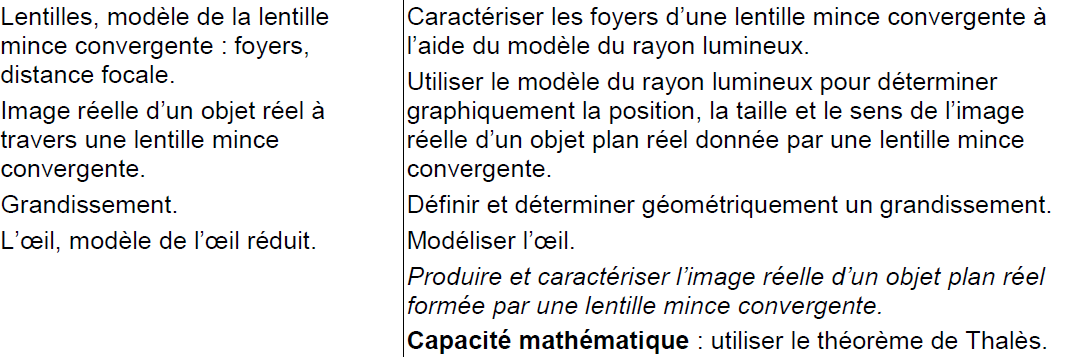
\includegraphics[width=.95\textwidth]{BO.png}
\end{center}
}


\doc{2}{Exercices dans le livre scolaire}{
		\begin{enumerate}
			\item Compétence de base : exercice 16 page 296
			\item Pour confirmer vos compétences : exercice 17page 296
			\item Parcours expert exercice 29 page 299
		\end{enumerate}
}
	\noindent \textbf{Quiz sur les lentilles}
\begin{center}
	\begin{minipage}{.25\textwidth}
		\centering
		
\includegraphics[width=.7\textwidth]{Quiz1.png}
		
		Quiz 1 - Caractéristique des lentilles : \url{https://forms.office.com/r/QuV6DC7PKj?origin=lprLink}
	\end{minipage}\hspace{1cm}
	\begin{minipage}{.25\textwidth}
		\centering
		
\includegraphics[width=.7\textwidth]{Quiz2.png}

		Quiz 2 - Construction d'une image à travers une lentille: \url{https://forms.office.com/r/hp3Y8X4W3q?origin=lprLink}
	\end{minipage}\hspace{1cm}
\begin{minipage}{.25\textwidth}
			\centering
			
\includegraphics[width=.7\textwidth]{Quiz3.png}
	
			Quiz 3 - Modèle optique de l'oeil: \url{https://forms.office.com/r/umt7L00HTe?origin=lprLink}
		\end{minipage}
\end{center}

\clearpage
\section*{Introduction}

Au cours de ce chapitre, nous nous intéresserons à l'étude de dispositif optiques qui jouent un rôle essentiel dans notre quotidien. Des lunettes qui améliorent notre vision aux appareils photos qui capturent des moments précieux. Les lentilles sont omniprésentes et influencent notre perception du monde qui nous entoure.\medskip

\begin{figure}[ht]
	\centering
	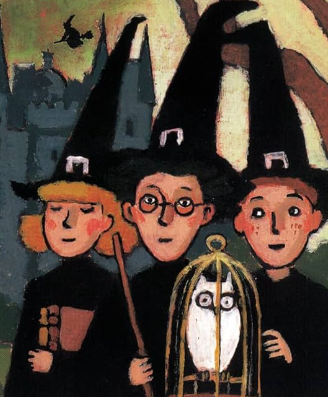
\includegraphics[width=.15\textwidth]{LunettesHarryPotter.png}\hspace{2cm}
	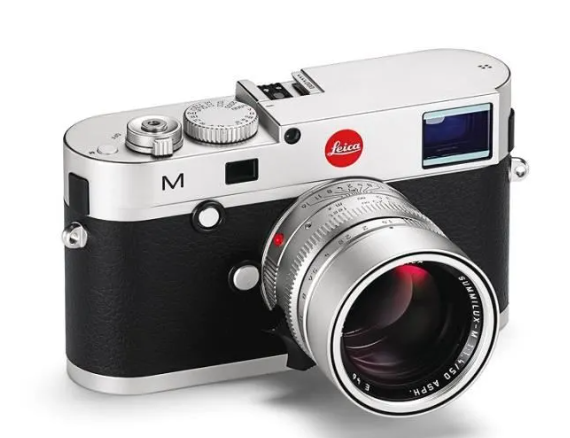
\includegraphics[width=.25\textwidth]{Leica.png}
	\caption{À gauche la couverture du premier livre d'Harry Potter avec ses lunettes rondes, à droite un appareil photo célèbre avec ses optiques.}
\end{figure}

Dans un premier temps nous présenteront les différents types de lentille, la modélisation de la lentille convergente et de l'\oe il que l'on étudiera du point de vue de l'opticien.
\section{Les différents types de lentilles et leur modélisation}

\subsection{Les lentilles minces}

\begin{center}
	\textit{reférence : le livre scolaire}
\end{center}

\begin{definition}{Définition 1 - lentille}
	Une lentille est un milieu transparent et homogène limité par deux surfaces appelées \textbf{dioptres} dont au moins une n'est pas plane.
\end{definition}

Le milieu qui constitue la lentille, en générale du verre est caractérisé par son \textbf{indice de réfraction}. Un rayon lumineux est dévié par \textbf{réfraction} à travers la lentille.

\subsection{On ditingue deux types de lentilles minces}

On distingue deux types de lentilles minces : les lentilles dites \textbf{convergentes} et \textbf{divergentes}.\medskip

\begin{minipage}{.6\textwidth}
\begin{Proposition}{Propriété 1 - lentilles convergentes}
	Les lentilles convergentes sont très minces aux bords et plus épaisses au centre.\medskip
	
	Un faisceau de lumière incident parallèle émerge de cette lentulle en un point : on dit qu'il \textbf{converge}.

\end{Proposition}
\end{minipage}\hfill
\begin{minipage}{.3\textwidth}
	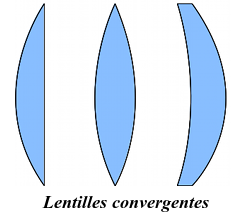
\includegraphics[width=.7\textwidth]{lentillecovnergente.png}
\end{minipage}\medskip

\begin{minipage}{.3\textwidth}
	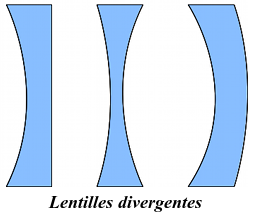
\includegraphics[width=.7\textwidth]{lentilledivergente.png}
\end{minipage}\hfill
\begin{minipage}{.6\textwidth}
	\begin{Proposition}{Propriété 2 - lentilles divergentes}
	Les lentilles divergentes ont les bords plus épais que leur centre.\medskip
	
	Un faisceau de lumière incident parallèle émerge de cette lentille en s'élargissant : on dit qu'il \textbf{diverge}.
\end{Proposition}
\end{minipage}

\clearpage
\subsection{La modéle de la lentille mince convergente}

On schématise les lentilles minces par une double flèche (représentant les vords fins). Toute lentille présente trois points caractéristiques : 

\begin{table}[ht]
	\centering
	% \resizebox{\textwidth}{!}{%
	\begin{tabular}{|c|p{12cm}|}
	\hline
	\rowcolor[HTML]{C0C0C0} 
	\textbf{Caractéristique}         & \textbf{Définition}   \\ \hline
	Centre optique noté $O$          & \begin{tabular}[c]{@{}l@{}} \makebox[12cm]{C'est le centre de la lentille mince. Les rayons } \\ \makebox[12cm]{ traversant la lentille en passant par ce point  ne sont pas déviés.} \end{tabular} \\ \hline
	Un foyer objet noté $F$          & \begin{tabular}[c]{@{}l@{}} \makebox[12cm]{Lorsqu'un rayon traverse une lentille en passant par son foyer objet,} \\ \makebox[12cm]{ il émerge de la lentille parallèle à l'axe optiqque de la lentille.} \end{tabular} \\ \hline
	Un foyer image noté $F^{\prime}$ & \begin{tabular}[c]{@{}l@{}} \makebox[12cm]{C'est le point symétrique de F par rapport à la lentille. Tout }\\ \makebox[12cm]{rayon incident parallèle à l'axe optique émerge en passant par $F^prime$} \end{tabular} \\ \hline
	\end{tabular}%
	% }
	\end{table}

	% \begin{table}[ht]
	% 	\centering
	% 	% \resizebox{\textwidth}{!}{%
	% 	\begin{tabular}{|c|p{12cm}|}
	% 	\hline
	% 	\rowcolor[HTML]{C0C0C0} 
	% 	\textbf{Caractéristique}         & \textbf{Définition}   \\ \hline
	% 	Centre optique noté $O$          & \begin{tabular}[c]{@{}l@{}} La partie centrale se réduit à un point appelé \\ centre optique et noté O\end{tabular} \\ \hline
	% 	Un foyer objet noté $F$          & \begin{tabular}[c]{@{}l@{}} Point symétrique du foyer image $F\prime$ par rapport à $O$. Tout faisceau \\ incident de lumière passant par $F$ émerge en un faisceau parallèle \\ à l'axe optique. \end{tabular} \\ \hline
	% 	Un foyer image noté $F^{\prime}$ & \begin{tabular}[c]{@{}l@{}} Point de convergence sur l'axe optique d'in faisceau incident de \\ lumière parallèle à l'axe optique. \end{tabular} \\ \hline
	% 	\end{tabular}%
	% 	% }
	% 	\end{table}

	\subsection{Dessins des rayons lumineux}

	\subsubsection{Rayon passant par le centre de la lentille}
	\begin{figure}[ht]
		\centering
		\begin{tikzpicture}[scale=.6]
			\filldraw[color =gray!10] (-1,-3)  rectangle (17,3);
			\draw[opacity = .3] (-1,-3) grid (17,3);
			\draw[ultra thick, ->] (0,0) -- (16,0) node[below]{Axe optique};
			\draw[ultra thick, <->] (8,-3) -- (8,3);
			\draw (7.5, -.5) node{$O$};
			% \draw[ultra thick, ->] (1,0) -- (1,2.5) node[left]{B};
			% \draw[ultra thick, red,  postaction={on each segment={mid arrow=red}}] (1,2.5) -- (8,2.5)-- (14,-2.2);
			\draw[ultra thick, red,  postaction={on each segment={mid arrow=red}}] (1,2.5) -- (8,0) -- (14,-2.2);
			% \draw[ultra thick, red,  postaction={on each segment={mid arrow=red}}] (1,2.5) -- (8,-2.2) -- (14,-2.2);
			
			\draw[ultra thick] (8-3.3, -.2) -- (8-3.3,.2);
			\draw[ultra thick] (3.3+8, -.2) -- (3.3+8,.2);
			% \draw[ultra thick] (1,-.5) node{A};
			\draw[ultra thick] (8-3.3,-.7) node{$F$};
			\draw[ultra thick] (8+3.3,-.7) node{$F\prime$};
			% \draw[ultra thick, ->] (14, 0) -- (14,-2.2) node[right]{B$\prime$};
			% \draw (14,.5) node{A$\prime$};
	
		\end{tikzpicture} 
	\end{figure}

	\begin{minipage}{.45\textwidth}
		\subsubsection{Rayon parallèle à l'axe optique traversant la lentille}


		% \begin{figure}[ht]
			\centering
			\begin{tikzpicture}[scale=.5]
				\filldraw[color =gray!10] (-1,-3)  rectangle (17,3);
				\draw[opacity = .3] (-1,-3) grid (17,3);
				\draw[ultra thick, ->] (0,0) -- (16,0) ;
				\draw[ultra thick, <->] (8,-3) -- (8,3);
				\draw (7.5, -.5) node{$O$};
				% \draw[ultra thick, ->] (1,0) -- (1,2.5) node[left]{B};
				\draw[ultra thick, red,  postaction={on each segment={mid arrow=red}}] (1,2.5) -- (8,2.5)-- (14,-2.2);
				% \draw[ultra thick, red,  postaction={on each segment={mid arrow=red}}] (1,2.5) -- (8,0) -- (14,-2.2);
				% \draw[ultra thick, red,  postaction={on each segment={mid arrow=red}}] (1,2.5) -- (8,-2.2) -- (14,-2.2);
				
				\draw[ultra thick] (8-3.3, -.2) -- (8-3.3,.2);
				\draw[ultra thick] (3.3+8, -.2) -- (3.3+8,.2);
				% \draw[ultra thick] (1,-.5) node{A};
				\draw[ultra thick] (8-3.3,-.7) node{$F$};
				\draw[ultra thick] (8+3.3,-.7) node{$F\prime$};
				% \draw[ultra thick, ->] (14, 0) -- (14,-2.2) node[right]{B$\prime$};
				% \draw (14,.5) node{A$\prime$};
		
			\end{tikzpicture} 
		% \end{figure}
	\end{minipage}\hfill
	\begin{minipage}{.45\textwidth}
		\subsubsection{Rayon passant par le foyer objet $F$ de la lentille}

		% \begin{figure}[ht]
			\centering
			\begin{tikzpicture}[scale=.5]
				\filldraw[color =gray!10] (-1,-3)  rectangle (17,3);
				\draw[opacity = .3] (-1,-3) grid (17,3);
				\draw[ultra thick, ->] (0,0) -- (16,0);
				\draw[ultra thick, <->] (8,-3) -- (8,3);
				\draw (7.5, -.5) node{$O$};
				% \draw[ultra thick, ->] (1,0) -- (1,2.5) node[left]{B};
				% \draw[ultra thick, red,  postaction={on each segment={mid arrow=red}}] (1,2.5) -- (8,2.5)-- (14,-2.2);
				% \draw[ultra thick, red,  postaction={on each segment={mid arrow=red}}] (1,2.5) -- (8,0) -- (14,-2.2);
				\draw[ultra thick, red,  postaction={on each segment={mid arrow=red}}] (1,2.5) -- (8,-2.2) -- (14,-2.2);
				
				\draw[ultra thick] (8-3.3, -.2) -- (8-3.3,.2);
				\draw[ultra thick] (3.3+8, -.2) -- (3.3+8,.2);
				% \draw[ultra thick] (1,-.5) node{A};
				\draw[ultra thick] (8-3.3,-.7) node{$F$};
				\draw[ultra thick] (8+3.3,-.7) node{$F\prime$};
				% \draw[ultra thick, ->] (14, 0) -- (14,-2.2) node[right]{B$\prime$};
				% \draw (14,.5) node{A$\prime$};
		
			\end{tikzpicture} 
		% \end{figure}
	\end{minipage}\bigskip

C'est ainsi que nous représentons en physique la trajectoir des rayons lumineux à travers les lentilles minces convergentes.

\clearpage
\section{Formation de l'image de l'objet AB à travers la lentille convergente}

\subsection{Construction de l'image d'un objet réel}

L'intersection des trois rayons lumineux issus de B et émergeants de la lentille définit l'image $B\prime$ du point B à travers la lentille. Le point image $A\prime$. du point A est l'intersection de l'axe optique et de la perpendiculaire à l'axe optique passant par $B\prime$.\medskip

\begin{definition}{Définition 2 - Image réelle et virtuelle}
	$\bullet$ L'image $\rm A^\prime B^\prime$ est dite \textbf{réelle} si elle formée après la lentille et donc observable sur un écran. Dans le cas contraire elle est dite \textbf{virtuelle}.
\end{definition}

\begin{definition}{Définition 3 - Image droite ou renversée}
	L'image est dite \textbf{renversée} lorsqu'elle est de sens opposé à celui de l'objet. Dans le cas contraire elle sera dite \textbf{droite}.
\end{definition}

\begin{figure}[ht]
	\centering
	\begin{tikzpicture}[scale=1]
		\filldraw[color =gray!10] (-1,-3)  rectangle (17,3);
		\draw[opacity = .3] (-1,-3) grid (17,3);
		\draw[ultra thick, ->] (0,0) -- (16,0) node[below]{Axe optique};
		\draw[ultra thick, <->] (8,-3) -- (8,3);
		\draw (7.5, -.5) node{$O$};
		\draw[ultra thick, ->] (1,0) -- (1,2.5) node[left]{B};
		\draw[ultra thick, red,  postaction={on each segment={mid arrow=red}}] (1,2.5) -- (8,2.5)-- (14,-2.2);
		\draw[ultra thick, red,  postaction={on each segment={mid arrow=red}}] (1,2.5) -- (8,0) -- (14,-2.2);
		\draw[ultra thick, red,  postaction={on each segment={mid arrow=red}}] (1,2.5) -- (8,-2.2) -- (14,-2.2);
		
		\draw[ultra thick] (8-3.3, -.2) -- (8-3.3,.2);
		\draw[ultra thick] (3.3+8, -.2) -- (3.3+8,.2);
		\draw[ultra thick] (1,-.5) node{A};
		\draw[ultra thick] (8-3.3,-.5) node{$F$};
		\draw[ultra thick] (8+3.3,-.5) node{$F\prime$};
		\draw[ultra thick, ->] (14, 0) -- (14,-2.2) node[right]{B$\prime$};
		\draw (14,.5) node{A$\prime$};

	\end{tikzpicture} 
\end{figure}

\subsection{Grandissment}

En général lorsque l'on forme une image d'un objet à l'aide d'une lentille sur un écran, l'image n'a pas la même taille que l'objet. La relation entre la taille de l'objet et de l'image est le grandissement:

\begin{definition}{Définition 4 - Grandissement}

	Le grandissement, noté $\gamma$ (\og{} gamma \fg{}), est le rapport entre la taille de l'image $A\prime B\prime$ et la taille de l'objet $AB$:

	\begin{equation}
		\gamma = \dfrac{\overline{A\prime B\prime }}{\overline{AB}}
	\end{equation}
\end{definition}

\begin{itemize}
	\item Si $\gamma < 0 $ alors l'image est renversée par rapport à l'objet 
	\item Si $\gamma >0$, on dit que l'image est droite.
	\item Si $|\gamma|>1$, alors l'image est agrandie par rapport à l'objet.
\end{itemize} 


\section{Modèle réduit de l'\oe il}
\begin{minipage}{.5\textwidth}
L'\oe il réel est un système optique complexe. Pour comprendre son fonctionnement d'un point de vue de l'optique on le modélise par un système plus simple comportant : \medskip

	\resizebox{.8\textwidth}{!}{%
	\begin{tabular}{|l|l|}
	\hline
	\rowcolor[HTML]{C0C0C0} 
	\textbf{Oeil réel} & \textbf{Modèle de l'oeil} \\ \hline
	Iris               &      Diaphragme          \\ \hline
	Cristallin         & Lentille convergente \\ \hline
	Rétine             & Écran     \\ \hline
	\end{tabular}%
	}
\end{minipage}
\begin{minipage}{.5\textwidth}
	\includegraphics*[width=1\textwidth]{oeil.png}
	\captionof{figure}{Modèle réduit de l' \oe il.}
	% 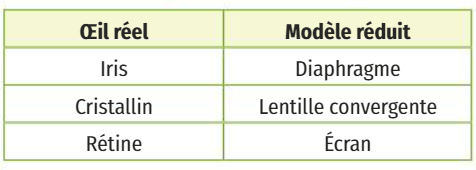
\includegraphics[width=.4\textwidth]{tableauOeil.png}
	% \caption{Représentation simplifiée de l'\oe il. \textit{ref:Le livre scolaire}}
\end{minipage}

\exo{2}{Accomodation de l'\oe il. Un \oe il emmétrope est capable de voir nettement des objets très éloignés ou très proches.}{
\analyser Le diamètre de l'\oe il est fixe, pour \textbf{accomoder}, c'est à dire pour former l'image de l'objet observé sur la rétine de l'\oe il que peut-on faire varier ? \medskip
	
L'oeil peut faire varier la courbure du cristallin, ce qui a pour conséauence de modifier la distance focale. Cette propriété permet \og{}d'accomoder\fg{} pour former l'image sur la rétine de l'\oe il.
}

\section{L'\oe il de votre smartphone}

\begin{figure}[ht]
	\centering
	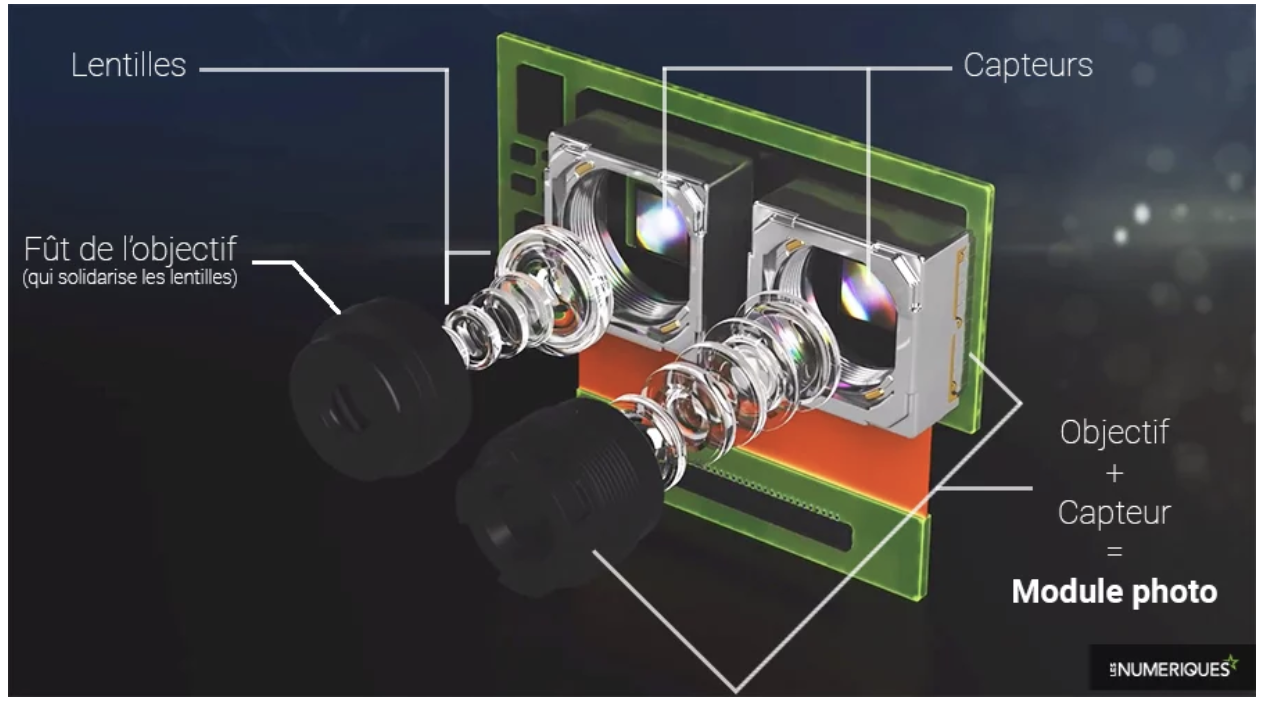
\includegraphics[width=.5\textwidth]{OeilPhotographique.png}
	\caption{Le capteur photographique du smartphone}
\end{figure}

\end{document}

%%
%% FIN DU DOCUMENT
%%
